\chapter{大整数运算}
在32位CPU下,C/C++中的int能表示的范围是$[-2^{32}, 2^{32}-1]$,unsigned int能表示的范围是$[0, 2^{32}]$。所以,int 和 unsigned int都不能保存超过 10位的整数(解方程$10^x \leq 2^{32}$,可得$x \leq 9.63$)。有时我们需要参与运算的整数,可能会远远不止10位,我们称这种基本数据类型无法表示的整数为大整数。如何表示和存放大整数呢?基本的思想是:用数组模拟大整数。一个数组元素,存放大整数中的一位。

例如,一个200位的十进制整数,可以用 \fn{int x[200]}来表示,一个数组元素对应一个位。这样做有点浪费空间,因为一个int可以表示的范围远远大于10。因此,我们可以用一个数组元素,表示4个数位(一个int可以表示的范围也远远大于10000,为什么一个数组元素只表示4个数位,可不可以表示9个数位?留给读者思考),这时,数组不再是10进制,而是10000进制。使用万进制,数组长度可以缩减到原来的1/4。

\section{大整数加法} %%%%%%%%%%%%%%%%%%%%%%%%%%%%%%
\subsubsection{描述}
求两个非负的大整数相加的和。

\subsubsection{输入}
有两行,每行是一个不超过200位的非负整数,可能有多余的前导0。

\subsubsection{输出}
一行,即相加后的结果。结果里不能有多余的前导0,即如果结果是342,那么就不能输出为0342。

\subsubsection{样例输入}
\begin{Code}
22222222222222222222 
33333333333333333333
\end{Code}

\subsubsection{样例输出}
\begin{Code}
55555555555555555555
\end{Code}

\subsubsection{代码}
\begin{Codex}[label=bigint_add.c]
#include<stdio.h>
#include<string.h>

/* 一个数组元素表示4个十进制位,即数组是万进制的 */
#define BIGINT_RADIX 10000
#define RADIX_LEN 4
#define MAX_LEN (200/RADIX_LEN+1)  /* 整数的最大位数 */

char    a[MAX_LEN * RADIX_LEN], b[MAX_LEN * RADIX_LEN];
int     x[MAX_LEN], y[MAX_LEN], z[MAX_LEN + 1];

/**
 * @brief 打印大整数.
 * @param[in] x 大整数,用数组表示,低位在低地址
 * @param[in] n 数组x的长度
 * @return 无
 */
void bigint_print(const int x[], const int n) {
    int i;
    int start_output = 0;  /* 用于跳过前导0 */
    for (i = n - 1; i >= 0; --i) {
        if (start_output) {  /* 如果多余的0已经都跳过,则输出 */
            printf("%04d", x[i]);
        } else if (x[i] > 0) {
            printf("%d", x[i]);
            start_output = 1; /* 碰到第一个非0的值,就说明多余的0已经都跳过 */
        }
    }

    if(!start_output) printf("0");  /* 当x全为0时 */
}

/**
 * @brief 将输入的字符串转化为大整数.
 * @param[in] s 输入的字符串
 * @param[out] x 大整数,用数组表示,低位在低地址
 * @return 无
 */
void bigint_input(const char s[], int x[]) {
    int i, j = 0;
    const int len = strlen(s);
    for (i = 0; i < MAX_LEN; i++) x[i] = 0;

    // for (i = len - 1; i >= 0; i--) a[j++] = s[i] - '0';
    for (i = len; i > 0; i -= RADIX_LEN) {  /* [i-RADIX_LEN, i) */
        int temp = 0;
        int k;
        const int low = i-RADIX_LEN > 0 ? i-RADIX_LEN : 0;
        for (k = low; k < i; k++) {
            temp = temp * 10 + s[k] - '0';
        }

        x[j++] = temp;
    }
}

/**
 * @brief 大整数加法
 * @param[in] x x
 * @param[in] y y
 * @param[out] z z=x+y
 * @return 无
 */
void bigint_add(const int x[], const int y[], int z[]) {
    int i;
    for (i = 0; i < MAX_LEN + 1; i++) z[i] = 0;

    for (i = 0; i < MAX_LEN; i++) {  /* 逐位相加 */
        z[i] += x[i] + y[i];
        if (z[i] >= BIGINT_RADIX) {  /* 看是否要进位 */
            z[i] -= BIGINT_RADIX;
            z[i+1] ++;  /* 进位 */
        }
    }
}


int main() {
    scanf("%s%s", a, b);

    bigint_input(a, x);
    bigint_input(b, y);

    bigint_add(x, y, z);
    bigint_print(z, MAX_LEN + 1);
    printf("\n"); 
    return 0;
}
\end{Codex}

\subsubsection{相关的题目}
与本题相同的题目:
\begindot
\item 《程序设计导引及在线实践》\footnote{李文新,程序设计导引及在线实践, 清华大学出版社, 2007}第144页7.1节
\item 百练 2981 大整数加法, \myurl{http://poj.grids.cn/practice/2981/}
\myenddot

与本题相似的题目:
\begindot
\item  TODO
\myenddot


\section{大整数减法} %%%%%%%%%%%%%%%%%%%%%%%%%%%%%%
\subsubsection{描述}
求两个非负的大整数相减的差。

\subsubsection{输入}
第1行是测试数据的组数T,每组测试数据占2行,第1行是被减数a,第2行是减数b(a > b),每行数据不超过100个字符,没有多余的前导0。每组测试数据之间有一个空行。

\subsubsection{输出}
每组测试数据输出一行,即相应的差

\subsubsection{样例输入}
\begin{Code}
2
9999999999999999999999999999999999999
9999999999999

5409656775097850895687056798068970934546546575676768678435435345
1
\end{Code}

\subsubsection{分析}
模拟小学生列竖式做加法,从个位开始逐位相加,超过或达到10(这里用万进制,则是10000)则进位。

两个200位的大整数相加,结果可能会有201位。

\subsubsection{样例输出}
\begin{Code}
9999999999999999999999990000000000000
5409656775097850895687056798068970934546546575676768678435435344
\end{Code}

\subsubsection{代码}
\begin{Codex}[label=bigint_sub.c]
#include<stdio.h>
#include<string.h>

/* 一个数组元素表示4个十进制位,即数组是万进制的 */
#define BIGINT_RADIX 10000
#define RADIX_LEN 4
#define MAX_LEN (100/RADIX_LEN+1)  /* 整数的最大位数 */

char    a[MAX_LEN * RADIX_LEN], b[MAX_LEN * RADIX_LEN];
int     x[MAX_LEN], y[MAX_LEN], z[MAX_LEN];

/**
 * @brief 打印大整数.
 * @param[in] x 大整数,用数组表示,低位在低地址
 * @param[in] n 数组x的长度
 * @return 无
 */
void bigint_print(const int x[], const int n) {
    int i;
    int start_output = 0;  /* 用于跳过前导0 */
    for (i = n - 1; i >= 0; --i) {
        if (start_output) {  /* 如果多余的0已经都跳过,则输出 */
            printf("%04d", x[i]);
        } else if (x[i] > 0) {
            printf("%d", x[i]);
            start_output = 1; /* 碰到第一个非0的值,就说明多余的0已经都跳过 */
        }
    }

    if(!start_output) printf("0");  /* 当x全为0时 */
}

/**
 * @brief 将输入的字符串转化为大整数.
 * @param[in] s 输入的字符串
 * @param[out] x 大整数,用数组表示,低位在低地址
 * @return 无
 */
void bigint_input(const char s[], int x[]) {
    int i, j = 0;
    const int len = strlen(s);
    for (i = 0; i < MAX_LEN; i++) x[i] = 0;

    // for (i = len - 1; i >= 0; i--) a[j++] = s[i] - '0';
    for (i = len; i > 0; i -= RADIX_LEN) {  /* [i-RADIX_LEN, i) */
        int temp = 0;
        int k;
        const int low = i-RADIX_LEN > 0 ? i-RADIX_LEN : 0;
        for (k = low; k < i; k++) {
            temp = temp * 10 + s[k] - '0';
        }

        x[j++] = temp;
    }
}

/**
 * @brief 大整数减法.
 *
 * @param[in] x x
 * @param[in] y y, x>y
 * @param[out] z z=x-y
 * @return 无
 */
void bigint_sub(const int x[], const int y[], int z[]) {
    int i;
    for (i = 0; i < MAX_LEN; i++) z[i] = 0;

    for (i = 0; i < MAX_LEN; i++) {  /* 逐位相减 */
        z[i] += x[i] - y[i];
        if (z[i] < 0) {  /* 看是否要借位 */
            z[i] += BIGINT_RADIX;
            z[i+1] --;  /* 借位 */
        }
    }
}

int main() {
    int T;    
    scanf("%d", &T);

    while (T-- > 0) {
        scanf("%s%s",a,b);

        bigint_input(a, x);
        bigint_input(b, y);

        bigint_sub(x, y, z);
        bigint_print(z, MAX_LEN);
        printf("\n"); 
    }
    return 0;
}
\end{Codex}

\subsubsection{相关的题目}
与本题相同的题目:
\begindot
\item 百练 2736 大整数减法, \myurl{http://poj.grids.cn/practice/2736/}
\myenddot

与本题相似的题目:
\begindot
\item  TODO
\myenddot


\section{大整数乘法} %%%%%%%%%%%%%%%%%%%%%%%%%%%%%%
\label{sec:bigintmul}
\subsubsection{描述}
求两个非负的大整数相乘的积。

\subsubsection{输入}
有两行,每行是一个不超过200位的非负整数,没有多余的前导0。 

\subsubsection{输出}
一行,即相乘后的结果。结果里不能有多余的前导0。 

\subsubsection{样例输入}
\begin{Code}
12345678900
98765432100
\end{Code}

\subsubsection{样例输出}
\begin{Code}
1219326311126352690000
\end{Code}

\subsubsection{分析}
两个200位的数相乘,积最多会有400位。

计算的过程基本上和小学生列竖式做乘法相同。为编程方便,并不急于处理进位,而将进位问题留待最后统一处理。 

现以$835 \times 49$为例来说明程序的计算过程。

先算$835 \times9$。$5 \times 9$得到45个1 ,$3 \times 9$ 得到27 个10,$8 \times 9$ 得到 72个100。由于不急于处理进位,所以$835 \times 9$ 算完后,aResult 如下:
\begin{center}
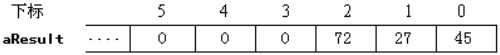
\includegraphics[width=260pt]{bigintmul1.png}\\
\end{center}

接下来算$4 \times 5$ 。此处$4 \times 5$的结果代表20个10 ,因此要 aResult[1]+=20,变为:
\begin{center}
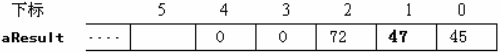
\includegraphics[width=260pt]{bigintmul2.png}\\
\end{center}

再下来算$4 \times 3$。此处$4 \times 3$的结果代表12个100,因此要 aResult[2]+= 12,变为:
\begin{center}
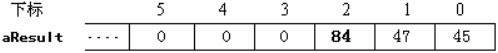
\includegraphics[width=260pt]{bigintmul3.png}\\
\end{center}

最后算$4 \times 8$。此处$4 \times 8$的结果代表32个1000 ,因此要 aResult[3]+= 32,变为:
\begin{center}
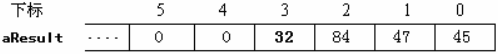
\includegraphics[width=260pt]{bigintmul4.png}\\
\end{center}

乘法过程完毕。接下来从 aResult[0] 开始向高位逐位处理进位问题。aResult[0]留下5,把4 加到aResult[1]上,aResult[1]变为 51 后,应留下 1 ,把5 加到aResult[2]上……最终使得aResult 里的每个元素都是 1 位数,结果就算出来了:
\begin{center}
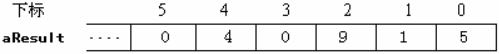
\includegraphics[width=260pt]{bigintmul5.png}\\
\end{center}

总结一个规律,即一个数的第i位和另一个数的第j位相乘所得的数,一定是要累加到结果的第i+j位上。这里i, j都是从右往左,从0开始数。

\subsubsection{代码}
\begin{Codex}[label=bigint_mul.c]
#include<stdio.h>
#include<string.h>

/* 一个数组元素表示4个十进制位,即数组是万进制的 */
#define BIGINT_RADIX 10000
#define RADIX_LEN 4
#define MAX_LEN (200/RADIX_LEN+1)  /* 整数的最大位数 */

char    a[MAX_LEN * RADIX_LEN], b[MAX_LEN * RADIX_LEN];
int     x[MAX_LEN], y[MAX_LEN], z[MAX_LEN * 2];

/**
 * @brief 打印大整数.
 * @param[in] x 大整数,用数组表示,低位在低地址
 * @param[in] n 数组x的长度
 * @return 无
 */
void bigint_print(const int x[], const int n) {
    int i;
    int start_output = 0;  /* 用于跳过前导0 */
    for (i = n - 1; i >= 0; --i) {
        if (start_output) {  /* 如果多余的0已经都跳过,则输出 */
            printf("%04d", x[i]);
        } else if (x[i] > 0) {
            printf("%d", x[i]);
            start_output = 1; /* 碰到第一个非0的值,就说明多余的0已经都跳过 */
        }
    }

    if(!start_output) printf("0");  /* 当x全为0时 */
}

/**
 * @brief 将输入的字符串转化为大整数.
 * @param[in] s 输入的字符串
 * @param[out] x 大整数,用数组表示,低位在低地址
 * @return 无
 */
void bigint_input(const char s[], int x[]) {
    int i, j = 0;
    const int len = strlen(s);
    for (i = 0; i < MAX_LEN; i++) x[i] = 0;

    // for (i = len - 1; i >= 0; i--) a[j++] = s[i] - '0';
    for (i = len; i > 0; i -= RADIX_LEN) {  /* [i-RADIX_LEN, i) */
        int temp = 0;
        int k;
        const int low = i-RADIX_LEN > 0 ? i-RADIX_LEN : 0;
        for (k = low; k < i; k++) {
            temp = temp * 10 + s[k] - '0';
        }

        x[j++] = temp;
    }
}

/**
 * @brief 大整数乘法.
 * @param[in] x x
 * @param[in] y y
 * @param[out] z z=x*y
 * @return 无
 */
void bigint_mul(const int x[], const int y[], int z[]) {
    int i, j;
    for (i = 0; i < MAX_LEN * 2; i++) z[i] = 0;

    for (i = 0; i < MAX_LEN; i++) {
        for (j = 0; j < MAX_LEN; j++) { /*用y[i],去乘以x的各位*/
            z[i + j] += y[i] * x[j]; /* 两数第i, j位相乘,累加到结果的第i+j位 */

            if (z[i + j] >= BIGINT_RADIX) { /* 看是否要进位 */
                z[i + j + 1] += z[i + j] / BIGINT_RADIX; /* 进位 */
                z[i + j] %= BIGINT_RADIX;
            }
        }
    }
}


int main() {
    scanf("%s%s", a, b);

    bigint_input(a, x);
    bigint_input(b, y);

    bigint_mul(x, y, z);
    bigint_print(z, MAX_LEN * 2);
    printf("\n");
    return 0;
}
\end{Codex}

\subsubsection{相关的题目}
与本题相同的题目:
\begindot
\item 《程序设计导引及在线实践》\footnote{李文新,程序设计导引及在线实践, 清华大学出版社, 2007}第146页7.2节
\item 百练 2980 大整数乘法, \myurl{http://poj.grids.cn/practice/2980/}
\myenddot

与本题相似的题目:
\begindot
\item  TODO
\myenddot


\section{大整数除法} %%%%%%%%%%%%%%%%%%%%%%%%%%%%%%
\subsubsection{描述}
求两个非负的大整数相除的商。

\subsubsection{输入}
第1行是测试数据的组数T,每组测试数据占2行,第1行是被除数,第2行是除数,每行数据不超过100 个字符。每组测试数据之间有一个空行。

\subsubsection{输出}
每组测试数据输出一行,即相应的整数商

\subsubsection{样例输入}
\begin{Code}
3
2405337312963373359009260457742057439230496493930355595797660791082739646
2987192585318701752584429931160870372907079248971095012509790550883793197894

10000000000000000000000000000000000000000
10000000000

5409656775097850895687056798068970934546546575676768678435435345
1
\end{Code}

\subsubsection{样例输出}
\begin{Code}
0
1000000000000000000000000000000
5409656775097850895687056798068970934546546575676768678435435345
\end{Code}

\subsubsection{分析}
基本的思想是反复做减法,看看从被除数里最多能减去多少个除数,商就是多少。一个一个减显然太慢,如何减得更快一些呢?以 7546 除以23为例来看一下:开始商为0。先减去23的100倍,就是2300,发现够减3次,余下646。于是商的值就增加300。然后用646减去230,发现够减 2 次,余下 186,于是商的值增加20。最后用186减去23,够减8次,因此最终商就是328。

所以本题的核心是要写一个大整数的减法函数,然后反复调用该函数进行减法操作。

计算除数的10倍、100倍的时候,不用做乘法,直接在除数后面补0即可。

\subsubsection{代码}
\begin{Codex}[label=bigint_div.c]
#include <stdio.h>
#include <stdlib.h>
#include <string.h>

/* 一个数组元素表示4个十进制位,即数组是万进制的 */
#define BIGINT_RADIX 10000
#define RADIX_LEN 4
#define MAX_LEN (100/RADIX_LEN+1)  /* 整数的最大位数 */

char    a[MAX_LEN * RADIX_LEN], b[MAX_LEN * RADIX_LEN];
int     x[MAX_LEN], y[MAX_LEN], z[MAX_LEN];

/**
 * @brief 打印大整数.
 * @param[in] x 大整数,用数组表示,低位在低地址
 * @param[in] n 数组x的长度
 * @return 无
 */
void bigint_print(const int x[], const int n) {
    int i;
    int start_output = 0;  /* 用于跳过前导0 */
    for (i = n - 1; i >= 0; --i) {
        if (start_output) {  /* 如果多余的0已经都跳过,则输出 */
            printf("%04d", x[i]);
        } else if (x[i] > 0) {
            printf("%d", x[i]);
            start_output = 1; /* 碰到第一个非0的值,就说明多余的0已经都跳过 */
        }
    }

    if(!start_output) printf("0");  /* 当x全为0时 */
}

/**
 * @brief 将输入的字符串转化为大整数.
 * @param[in] s 输入的字符串
 * @param[out] x 大整数,用数组表示,低位在低地址
 * @return 无
 */
void bigint_input(const char s[], int x[]) {
    int i, j = 0;
    const int len = strlen(s);
    for (i = 0; i < MAX_LEN; i++) x[i] = 0;

    // for (i = len - 1; i >= 0; i--) a[j++] = s[i] - '0';
    for (i = len; i > 0; i -= RADIX_LEN) {  /* [i-RADIX_LEN, i) */
        int temp = 0;
        int k;
        const int low = i-RADIX_LEN > 0 ? i-RADIX_LEN : 0;
        for (k = low; k < i; k++) {
            temp = temp * 10 + s[k] - '0';
        }

        x[j++] = temp;
    }
}

/**
 * @brief 计算大整数的位数.
 *
 * @param[inout] x 大整数
 * @return 位数
 */
static int length(const int x[]) {
    int i;
    int result = 0;
    for (i = MAX_LEN - 1; i >= 0; i--) if (x[i] > 0) {
        result = i + 1;
        break;
    }
    return result;
}

/**
 * @brief 大整数减法.
 *
 * @param[inout] x x
 * @param[in] y y
 * @return 如果x < y,返回-1,如果x=y,返回0,如果x>y,返回1
 */
static int bigint_sub(int x[], const int y[]) {
    int i;
    const int lenx = length(x);
    const int leny = length(y);

    /* 判断x是否比y大 */
    if (lenx < leny) return -1;
    else if (lenx == leny) {
        int larger = 0;
        for (i = lenx - 1; i >= 0; i--) {
            if (x[i] > y[i]) {
                larger = 1;
            } else if (x[i] < y[i]) {
                if (!larger) return -1;
            }
        }
    }
    
    for (i = 0; i < MAX_LEN; i++) {  /* 逐位相减 */
        x[i] -= y[i];
        if (x[i] < 0) {  /* 看是否要借位 */
            x[i] += BIGINT_RADIX;
            x[i+1] --;  /* 借位 */
        }
    }

    return 1;
}

/**
 * @brief 大整数除法.
 *
 * @param[inout] x x
 * @param[in] y y
 * @param[out] z z=x/y
 * @return 无
 */
void bigint_div(int x[], const int y[], int z[]) {
    int i;
    int *yy; /* y的副本 */
    const int xlen = length(x);
    int ylen = length(y);
    const int times = xlen - ylen;

    for (i = 0; i < MAX_LEN; i++) z[i] = 0;
    if (times < 0) return;

    yy = (int*)malloc(sizeof(int) * MAX_LEN);
    memcpy(yy, y, sizeof(int) * MAX_LEN);


    /* 将yy右移times位,使其长度和x相同,即 yy 乘以 10000 的times次幂 */
    for (i = xlen - 1; i >= 0; i--) {
        if (i >= times) yy[i] = yy[i - times];
        else yy[i] = 0;
    }

    /* 先减去若干个 y×(10000的 times次方), 
      不够减了,再减去若干个 y×(10000的 times-1次方)
      一直减到不够减为止 */
    ylen = xlen;
    for (i = 0; i <= times; i++) {
        int j;
        while (bigint_sub(x, yy) >= 0) {
            z[times - i]++;
        }

        /* yy 除以BIGINT_RADIX,即左移一位 */
        for (j = 1; j < ylen; j++) {
            yy[j - 1] = yy[j];
        }
        yy[--ylen] = 0;
    }

    /* 下面的循环统一处理进位 */
    for (i = 0; i < MAX_LEN - 1; i++) {
        if (z[i] >= BIGINT_RADIX) {  /* 看是否要进位 */
            z[i+1] += z[i] / BIGINT_RADIX;  /* 进位 */
            z[i] %= BIGINT_RADIX;
        }
    }
    free(yy);
}

int main() {
    int T;    
    scanf("%d", &T);

    while (T-- > 0) {
        scanf("%s%s",a,b);

        bigint_input(a, x);
        bigint_input(b, y);

        bigint_div(x, y, z);
        bigint_print(z, MAX_LEN);
        printf("\n"); 
    }
    return 0;
}
\end{Codex}

\subsubsection{相关的题目}
与本题相同的题目:
\begindot
\item 《程序设计导引及在线实践》\footnote{李文新,程序设计导引及在线实践, 清华大学出版社, 2007}第149页7.3节
\item 百练 2737 大整数除法, \myurl{http://poj.grids.cn/practice/2737/}
\item wikioi 3118 高精度练习之除法 , \myurl{http://poj.grids.cn/practice/3118/}
\myenddot

与本题相似的题目:
\begindot
\item  TODO
\myenddot


\section{大数阶乘} %%%%%%%%%%%%%%%%%%%%%%%%%%%%%%

\subsection{大数阶乘的位数} %%%%%%%%%%%%%%%%%%%%%%%%%%%%%%
\subsubsection{描述}
求$n!$的位数, $0 \leq n \leq 10^7$。

\subsubsection{输入}
第一行是一个正整数$T$,表示测试用例的个数。接下来的$T$行,每行一个正整数$n$。

\subsubsection{输出}
对每个$n$,每行输出$n!$的位数

\subsubsection{样例输入}
\begin{Code}
2
10
20
\end{Code}

\subsubsection{样例输出}
\begin{Code}
7
19
\end{Code}

\subsubsection{分析}
最简单的办法,是老老实实计算出$n!$,然后就知道它的位数了。但这个方法很慢,会超时(TLE)。

组合数学里有个Stirling公式(Stirling's formula\footnote{\myurl{http://en.wikipedia.org/wiki/Stirling's_approximation}}):
$$
\lim_{n \to \infty}{\dfrac{n!}{\sqrt{2\pi n}\left(\frac{n}{e} \right)^n}}=1
$$

可以用这个公式来计算$n!$的位数,它等于
$$
n\log{\dfrac{n}{e}}+\dfrac{1}{2}\log{2\pi n}+1
$$

\subsubsection{代码}
\begin{Codex}[label=bigint_factorial_digits.c]
#include <stdio.h>
#include <math.h>

/**
 * @brief 计算n的阶乘的位数,用Stirling公式
 * @param[in] n n>=0
 * @return n的阶乘的位数
 */
int factorial_digits(unsigned int n) {
    const double PI = 3.14159265358979323846;
    const double E = 2.7182818284590452354;
    if (n == 0) return 1;
    return (int)(n * log10(n/E) + 0.5 * log10(2*PI*n)) + 1;
}

int main() {
    int i, T, n;

    scanf("%d", &T);
    for (i = 0; i < T; i++) {
        scanf("%d", &n);
        printf("%d\n", factorial_digits(n));
    }
    return 0;
}
\end{Codex}

\subsubsection{相关的题目}
与本题相同的题目:
\begindot
\item POJ 1423 Big Number, \myurl{http://poj.org/problem?id=1423}
\myenddot

与本题相似的题目:
\begindot
\item  TODO
\myenddot


\subsection{大数阶乘} %%%%%%%%%%%%%%%%%%%%%%%%%%%%%%
\subsubsection{描述}
计算$n!, 0 \leq n \leq 10000)$。

\subsubsection{输入}
每行一个整数$n$

\subsubsection{输出}
对每个$n$,每行输出$n!$

\subsubsection{样例输入}
\begin{Code}
1
2
3
\end{Code}

\subsubsection{样例输出}
\begin{Code}
1
2
6
\end{Code}

\subsubsection{代码}
\begin{Codex}[label=bigint_factorial.c]
#include<stdio.h>
#include<string.h>

/* 一个数组元素表示4个十进制位,即数组是万进制的 */
#define BIGINT_RADIX 10000
#define RADIX_LEN 4
/* 10000! 有 35660 位 */
#define MAX_LEN (35660/RADIX_LEN+1)  /* 整数的最大位数 */

int     x[MAX_LEN + 1];

/**
 * @brief 打印大整数.
 * @param[in] x 大整数,用数组表示,低位在低地址
 * @param[in] n 数组x的长度
 * @return 无
 */
void bigint_print(const int x[], const int n) {
    int i;
    int start_output = 0;  /* 用于跳过前导0 */
    for (i = n - 1; i >= 0; --i) {
        if (start_output) {  /* 如果多余的0已经都跳过,则输出 */
            printf("%04d", x[i]);
        } else if (x[i] > 0) {
            printf("%d", x[i]);
            start_output = 1; /* 碰到第一个非0的值,就说明多余的0已经都跳过 */
        }
    }

    if(!start_output) printf("0");  /* 当x全为0时 */
}

/**
 * @brief 大整数乘法, x = x*y.
 * @param[inout] x x
 * @param[in] y y
 * @return 无
 */
void bigint_mul(int x[], const int y) {
    int i;
    int c = 0; /* 保存进位 */

    for (i = 0; i < MAX_LEN; i++) { /*用y,去乘以x的各位*/
        const int tmp = x[i] * y + c;
        x[i] = tmp % BIGINT_RADIX;
        c = tmp / BIGINT_RADIX;
    }
}

/**
 * @brief 计算n的阶乘
 * @param[in] n
 * @param[out] x 存放结果
 * @return 无
 */
void bigint_factorial(int n, int x[]) {
    int i;
    memset(x, 0, sizeof(int) * (MAX_LEN + 1));
    x[0] = 1;

    for (i = 2; i <= n; i++) {
        bigint_mul(x, i);
    }
}


int main() {
    int n;
    while (scanf("%d", &n) != EOF) {
        bigint_factorial(n, x);
        bigint_print(x, MAX_LEN + 1);
        printf("\n");
    }
    return 0;
}
\end{Codex}

\subsubsection{相关的题目}
与本题相同的题目:
\begindot
\item HDU 1042 N!, \myurl{http://acm.hdu.edu.cn/showproblem.php?pid=1042}
\myenddot

与本题相似的题目:
\begindot
\item  TODO
\myenddot
